\documentclass[10pt,letterpaper]{article}
\usepackage[utf8]{inputenc}
\usepackage[english]{babel}
\usepackage{amsmath}
\usepackage{amsfonts}
\usepackage{amssymb}
\usepackage{makeidx}

\usepackage{graphicx}
\graphicspath{ {./images/} }

\usepackage{lmodern}
\usepackage{kpfonts}
\usepackage{comment}
\usepackage{hyperref}
\hypersetup{
    colorlinks=true,
    linkcolor=blue,
    filecolor=magenta,      
    urlcolor=cyan,
    pdftitle={Overleaf Example},
    pdfpagemode=FullScreen,
    }
\usepackage[left=2cm,right=2cm,top=2cm,bottom=2cm]{geometry}
\title{\textbf{K Means}}
\author{Written by Chris Piech. Based on a handout by Andrew Ng.}
\date{June 22 2021}
\begin{document}
\begin{titlepage}
\maketitle\maketitle
\begin{flushleft}
\href{https://www.overleaf.com/learn}{Latex code ref https://www.overleaf.com/learn} \\
\href{https://stanford.edu/~cpiech/cs221/handouts/kmeans.html}{Algorithm content ref https://stanford.edu/~cpiech/cs221/handouts/kmeans.html}
\end{flushleft}
\end{titlepage}
\section{Basic Idea}
Say you are given a data set where each observed example has a set of features, but has no labels. Labels are an essential ingredient to a supervised algorithm like Support Vector Machines, which learns a hypothesis function to predict labels given features. So we can't run supervised learning. What can we do? \\

One of the most straightforward tasks we can perform on a data set without labels is to find groups of data in our dataset which are similar to one another -- what we call clusters.\\

K-Means is one of the most popular "clustering" algorithms. K-means stores $k$ centroids that it uses to define clusters. A point is considered to be in a particular cluster if it is closer to that cluster's centroid than any other centroid.\\

K-Means finds the best centroids by alternating between (1) assigning data points to clusters based on the current centroids (2) chosing centroids (points which are the center of a cluster) based on the current assignment of data points to clusters.\\

\begin{figure}[h]
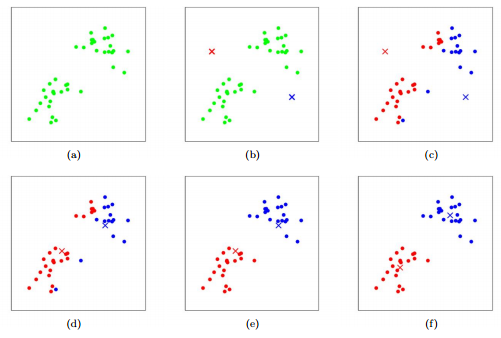
\includegraphics[scale=0.8]{kmeansViz.png}
\centering
\caption{K-means algorithm. Training examples are shown as dots, and cluster centroids are shown as crosses. (a) Original dataset. (b) Random initial cluster centroids. (c-f) Illustration of running two iterations of k-means. In each iteration, we assign each training example to the closest cluster centroid (shown by "painting" the training examples the same color as the cluster centroid to which is assigned); then we move each cluster centroid to the mean of the points assigned to it. Images courtesy of Michael Jordan.}
\label{figure1}
\end{figure}

\section{Algorithm}
In the clustering problem, we are given a training set ${x^{(1)}, ... , x^{(m)}}$, and want to group the data into a few cohesive "clusters." Here, we are given feature vectors for each data point $x^{(i)} \in \mathbb{R}^n$ as usual; but no labels $y^{(i)}$ (making this an unsupervised learning problem). Our goal is to predict $k$ centroids and a label $c^{(i)}$ for each datapoint. The k-means clustering algorithm is as follows:

\begin{itemize}
\item[1] Initialize \textbf{cluster centroids} $\mu_{1}, \mu_{2}, \ldots , \mu_{k} \in \mathbb{R}^{n}$ randomly.
\item[2] Repeat until convergence:{\\

		For every $i$, set \\
		$$c^(i):=arg \min_{j}$$
		}
\end{itemize}




\end{document}